\documentclass{apostila}
\graphicspath{{imgs/}} % Setting the graphicspath

\title{Git}
\author{Neni}
\date{\today}

\begin{document}
\chapter{O que é Git}


\chapter{Configurando ambiente}


\chapter{Conceitos}


\chapter{Uso básico}

\section{Individual}
\begin{figure}[h]
  \caption{Fluxo de trabalho básico do git}
  \centering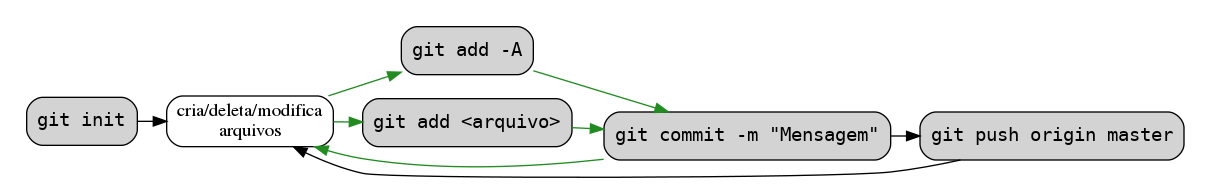
\includegraphics[width=\textwidth]{fluxo-simples.png}
\end{figure}
\subsection{Add}
\subsection{Commit}
\subsubsection{Mensagens de commits}
\subsection{Push}
\subsection{Tag}
\subsection{Rebase}

\section{Em time}
\subsection{Pull}
\subsection{Fetch}
\subsection{Branches}
\subsection{Merge}


\chapter{Fluxos de trabalho}
\section{Comum}
\section{Gitflow}
\section{Pessoal para estudos}


\chapter{Exemplos de cenários específicos}
\section{Exeplo 1}
\subsection{TLDR}
\subsection{Resolução}
\section{Exeplo 2}
\subsection{TLDR}
\subsection{Resolução}
\section{Exeplo 3}
\subsection{TLDR}
\subsection{Resolução}


\chapter{Configurações}
\section{Usuário}
\subsection{Gitconfig}
\subsubsection{User}
\subsubsection{Colors}
\subsubsection{Template}
\subsubsection{Alias}
\subsection{SSH}

\section{Projeto}
\subsection{Gitignore}
\subsection{Gitconfig}
\subsection{Remotos}
\subsubsection{Readme}
\subsubsection{Template de issue e PR}
\subsubsection{Licença}

\chapter{Ferramentas}
\section{Extensões de Editores/IDEs}
\subsection{Vim/Neovim}
\subsubsection{vim-fugitive}
\subsubsection{gv.vim}
\subsubsection{vim-gitgutter}

\section{GUI}
\end{document}
